\section{Formal Methods in Verification and Validation}
\label{sec:fm}
As the complexity of systems increase, the cost of development and validation consumes more time and resources than ever before; nevertheless, these processes are vital in safety critical systems when the loss of functionality of the system can result in loss of life. Authorities have put in place various thresholds for the likelihood of such events and it is the responsibility of the system developers to show that this is incredibly unlikely to occur~\cite{faaSA}. Utilizing the recent advancements in automated formal verification within the validation process has become essential to the certification of critical systems~\cite{deptOfDefense,standard1999,prasad2005survey}. This section provides a summary of the formal method techniques that are commonly used in the system development and safety assessment processes.

\subsection{Overview}
Formal validation and verification is a proof-based methodology used to assess the correctness of requirements, system design, and implementation. In the past, this has been performed through manual means, but with the advancement in automated theorem proving and other formal methods, automated formal analyses not only guarantees a higher degree of confidence, but also reduces the time (and thus cost) of carrying out the proofs of correctness. Techniques used in formal validation and verification include automated theorem proving, model checking, and abstract interpretation. 

\subsubsection{Formal Specification}
Formal specification process translates the informal system requirements into a mathematical logic to determine if the system design is correct~\cite{hinchey2012industrial}. This process guarantees an unambiguous description of the requirements which is not possible when using an informal natural language. This formal definition of system requirements includes the system design and its expected behavior as well as the assumptions on environment. A design or implementation can never be considered correct in isolation; it is only correct with respect to the specifications. The expected behavior, system design, and environmental assumptions change and are refined as the system goes through the various stages of development. 

\subsubsection{Formal Verification} 
Formal verification is the use of proof methods to show that given the environmental assumptions stated in the formal specification, the formal design of the system meets the requirements. The problem can be reduced to that of property checking: given a program $P$ and a specific property, does the program satisfy the given property~\cite{fitting2012first}. This is an undecidable problem because a program can be represented as an infinite state space. The problem is that of finding a finite set of predicates that support the specified property over an infinite state space. This is an undecidable problem; any algorithm searching for a solution to this problem may not terminate~\cite{clarke2018model}. The approaches used to provide these proofs are usually deductive methods or an exhaustive exploration of the model known as model checking. 

Model checking was introduced in the early 1980's and consists of exploring the states and transitions of a model~\cite{clarke1981design,queille1982specification}. By representing the system abstractly, the infinite state space is reduced to a finite model. This addresses the undecidability factor~\cite{d2008survey}. The proofs are generated over an abstract mathematical model of the system, such as finite state machines, labeled transition systems, or timed automata. It takes as input a model of a system and the properties written in propositional temporal logic, then explores the entire state space of the system to determine if the model violates the properties~\cite{clarke2018model,fraser2009testing}. In recent years, model checking takes advantage of abstraction techniques specific to a domain to consider multiple states or transitions in a single operation; this lessens computation time considerably~\cite{d2008survey}. Nevertheless, the biggest limiting factor of model checking is scalability and much of the recent research in this area attempts to address this problem~\cite{clarke2018model}.

Deductive methods of verification consists of generating proof obligations from the specifications of the system and using these obligations in a theorem prover setting. Automated theorem provers have the main objective to show that some statement (conjecture) is a logical consequence of other statements (the axioms and hypotheses). The rules of inference are given as are the set of axioms and hypotheses~\cite{d2008survey,fitting2012first}. Deductive methods of verification include automated theorem provers (e.g., Coq~\cite{coq}, Isabelle~\cite{isabelle}) and satisfiability modulo theories (e.g., SMTInterpol~\cite{smtInterpol}, Z3~\cite{z3}, Yices~\cite{yices}). 


 
\section{Satisfiability}
\label{sec:sat}
The Boolean Satisfiability (SAT) problem attempts to determine if there exists a total truth assignment to a given propositional formula, that evaluates to $true$. Generally, a propositional formula is any combination of the disjunction and conjunction of literals (as an example, $a$ and $\neg a$ are literals). For example, the proposition $a \land b$ is satisfiable; when $a$ and $b$ are assigned to $true$, the formula is satisfied.  On the other hand, the proposition $a \land \neg a$ is unsatisfiable; no such assignment can be found to satisfy both $a$ and $\neg a$. SAT solvers in work over a constraint system of propositional logic to determine satisfiability. Satisfiability Modulo Theories (SMT) solvers also address the SAT problem, but can work over propositional logic or predicate logic with quantifiers. An SMT solver works over a conjunction of literals, as is the case with SAT solvers, but the literals can be expressed as predicates over non-boolean variables, such as $x > 0$. A boolean literal can be satisfied with a finite number of possible assignments; this is not always the case with SMT formula.

\subsection{UNSAT Cores and Minimal Unsatisfiable Subsets}
A constraint system $C$ is an ordered set of $n$ abstract constraints $\{C_1, C_2, ..., C_n\}$ over a set of variables. The constraint $C_i$ restricts the allowed assignments of these variables in some way~\cite{liffiton2016fast}. Given a constraint system, we require some method of determining, for any subset $S \subseteq C$, whether $S$ is \textit{satisfiable} (SAT) or \textit{unsatisfiable} (UNSAT). Given a constraint system $C$, there are certain subsets of $C$ that are of interest in terms of satisfiability. %Definitions 2-4 are taken from research by Liffiton et. al.~\cite{liffiton2016fast}. 

For a given unsatisfiable problem, SAT solvers (and SMT solvers) attempt to provide proof of unsatisfiability by providing a subset of UNSAT clauses known as \textit{UNSAT cores}. In general, this is useful information to have regarding the constraint system in question. 

\begin{definition} A Minimal Unsatisfiable Subset (MUS) $M$ of a finite constraint system $C$ is a subset $M \subseteq C$ such that $M$ is unsatisfiable and $\forall c \in M$ : $M \setminus \{c\}$ is satisfiable. 
\end{definition}

\begin{definition} UNSAT core: Let $C$ be a finite set of constraints and $U \subseteq C$ an unsatisfiable subset. A constraint $c \in U$ is an UNSAT core for $U$ if $U \setminus \{c\}$ is satisfiable. A set of all unsatisfiability cores of $U$ constitute an MUS for $C$. 
\end{definition}

Intuitively, an MUS is the minimal explanation of the constraint systems infeasability and the UNSAT cores are the building blocks of the MUS. In recent years, a number of efficient algorithms have been introduced to find MUSs~\cite{liffiton2005max} and most of them focus on finding a single such subset~\cite{belov2012towards, belov2013core, belov2012muser2}. More recently, algorithms have been introduced that can find all such minimal unsatisfiable subsets~\cite{GhassabaniGW16, Ghassabani2017EfficientGO,bendik2018online}. 

\subsection{Inductive Validity Cores} Given a complex model, it is useful to extract traceability information related to the proof; in other words, which elements of the model were necessary to construct the proof. An algorithm was introduced by Ghassabani et al. to provide Inductive Validity Cores (IVC) as a way to determine which model elements are necessary for the inductive proofs of the safety properties for sequential systems~\cite{GhassabaniGW16}. Given a safety property of the system, a model checker is invoked to construct a proof of the property. The IVC generation algorithm extracts traceability information from the proof process and returns a minimal set of the model elements required in order to prove the property. Later research extended this algorithm in order to produce all minimal IVC elements (\aivcalg)~\cite{Ghassabani2017EfficientGO,bendik2018online}. 

The \aivcalg algorithm considers a constraint system consisting of the assumptions and contracts of system components and the negation of the safety property of interest (i.e. the top level event). It then collects all Minimal Unsatisfiable Subsets (MUSs) of this constraint system; these are the minimal explanations of the constraint systems infeasibility in terms of the \textit{negation} of the safety property. Equivalently, these are the minimal model elements necessary to prove the safety property. 

\subsection{Ordered Binary Decision Diagrams}
A Binary Decision Diagram (BDD) is a data structure used to encode Boolean formulae.
\begin{figure}[!htb]
        \center{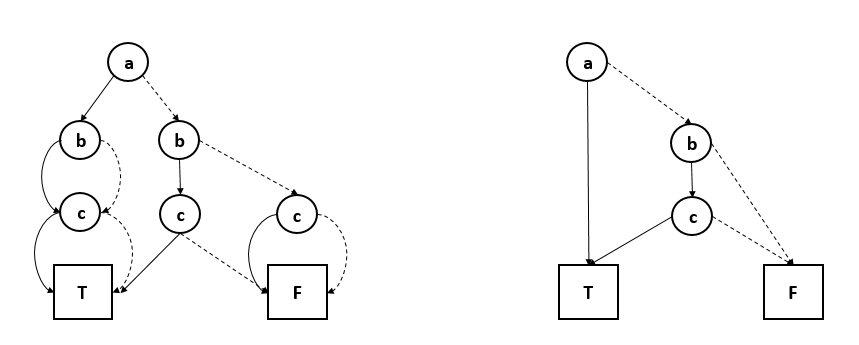
\includegraphics[width=0.8\textwidth] {images/bdd.png}}
        \caption{\label{fig:bdd} Binary Decision Diagrams of the Formula $a \lor (b \land c)$}
\end{figure}
As shown in Figure~\ref{fig:bdd}, it is a rooted, directed, acyclic graph with internal decision nodes and two terminal nodes (\textit{true} and \textit{false}). Each of the decision nodes is labeled with a Boolean variable and has two child nodes, low child and high child. The edge from a node to its low child represents the assignment of \textit{false}, likewise the edge to the high child represents the assignment of \textit{true}. The BDD is called \textit{ordered} if different variables appear in the same order on all paths from the root. Intuitively, following a path from the root to the \textit{true} terminal node represents a valid assignment to the Boolean formula (invalid in the case of ending on the \textit{false} terminal node). 

BDDs can also be reduced by the removal of isomorphic subgraphs. The BDD shown on the right of Figure~\ref{fig:bdd} is the reduced form of the BDD on the left. 












\subsection{Artifacts, Data Structures, and Other Formalizations}
\label{chap:artifacts}
The assessment processes of critical system development produce important artifacts that are used together for certification of the system, but those of importance to this thesis are \textit{Fault Trees} and associated sets called \textit{Minimal Cut Sets}. For this reason, more information is provided in this section on these artifacts.

\subsubsection{Fault Trees and Minimal Cut Sets}
The use of fault trees are common in many safety assessment processes and the ability to generate the cut sets needed for the construction of the fault tree is a useful part of any safety analysis tool. The fault tree is a safety artifact commonly referenced in requirement protocol documents such as ARP4761, ARP4754, and AIR6110~\cite{SAE:ARP4761,SAE:ARP4754A,AIR6110}.

A Fault Tree (FT) is a directed acyclic graph whose leaves model component failures and whose gates model failure propagation~\cite{0f356f05e72f43018211b36f97c8854a}. The system failure under examination is the root of the tree and is called the Top Level Event (TLE). The node types in a fault tree are \textit{events} and \textit{gates}. An event is an occurrence within the system, typically the failure of a subsystem down to an individual component. Events can be grouped into \textit{basic events} which occur independently, and \textit{intermediate events} which occur dependently and are caused by one or more other events~\cite{historyFTA}.  These events model the failure of the system (or subsystem) under consideration. The gates represent how failures propagate through the system and how failures in subsystems can cause system wide failures. The two most common logic symbols used in an FT are the Boolean logic AND-gates and OR-gates. An AND-gate is used when the undesired top level event can only occur when all the lower conditions are true. The OR-gate is used when the undesired event can occur if any one or more of the next lower conditions is true. This is not a comprehensive list of gate types; others include voting, inhibit, or negation gates~\cite{0f356f05e72f43018211b36f97c8854a}.
\begin{figure}[htbp]
\begin{center}
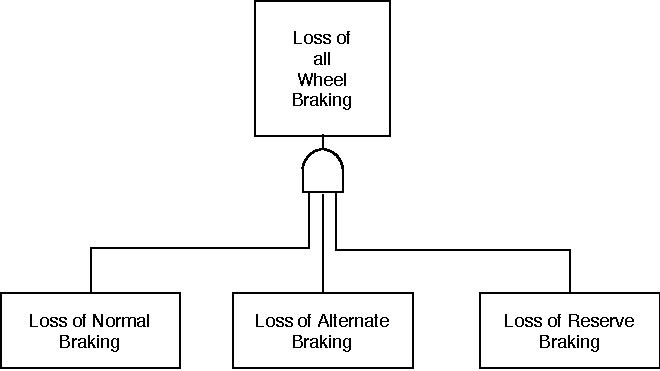
\includegraphics[width=8cm]{images/introFT2.pdf}
\caption{A simple fault tree} \label{fig:introFT}
\end{center}
\end{figure}

Figure~\ref{fig:introFT} shows a simple example of a fault tree based on SAE ARP4761~\cite{SAE:ARP4761}. In this example, the top level event corresponds to an aircraft losing all wheel braking. In order for this event to occur, all of the basic events must occur. This is seen through the use of the AND gate below the top level event. The gates in the fault tree describe how failures propagate through the system. Each gate has one output and one or more inputs. In Figure~\ref{fig:introFT}, the AND gate has three inputs and one output. The leaves of the tree represent the basic events of the system. %and 
In the case of this fault tree, these three events are also the Minimal Cut Sets (MinCutSets) for this top level event. A MinCutSet is the minimal set of basic events that must occur together in order to cause the TLE to occur. Generating and analyzing these MinCutSets is central to FTA and has been an active area of interest in the research community since fault trees were first described in Bell Labs in 1961~\cite{historyFTA,0f356f05e72f43018211b36f97c8854a}. 

There are two main types of fault tree analysis that we differentiate here as \textit{qualitative} analysis and \textit{quantitative} analysis. In qualitative analysis, the structure of the fault tree is considered and the MinCutSets are a way to indicate which combinations of component failures will cause the system to fail. On the other hand, in quantitative analysis, the probability of the TLE is calculated given the probability of occurrence of the basic events~\cite{0f356f05e72f43018211b36f97c8854a}. 

\subsubsection{Failure Mode and Effects Analysis}
\danielle{Is this section necessary? If I don't talk about FMEA tables again, cut this.} Failure Mode and Effects Analysis (FMEA) was one of the first systematic ways of performing dependability analysis and is used throughout the safety critical industries~\cite{rausand2003system,Bozzano:2011:SDP:1992983.1992988}. FMEA provides a structured way to list possible failures and their consequences systemwide. If probabilities of failures are known, quantitative analysis can be performed to estimate system reliability and to assign critical significance to potential failure modes or system components~\cite{MilStandardFMEA}. Performing FMEA is often the first step in the fault tree construction, for it shows possible component failures and hence basic events~\cite{0f356f05e72f43018211b36f97c8854a}. Typically, the failure modes of the components at a given level are considered; the objective it to identify the effects of the failure modes at that level - and usually higher levels - of the design. The FMEA results are often presented in tabular form (FMEA Table). FMEA tables vary in form, but almost always include failure mode definitions, the operational mode in which the failure can occur, and possible causes of the failure~\cite{Bozzano:2010:DSA:1951720}.

\subsubsection{Ordered Binary Decision Diagrams}
A Binary Decision Diagram (BDD) is a data structure used to encode Boolean formulae.
\begin{figure}[htbp]
        \center{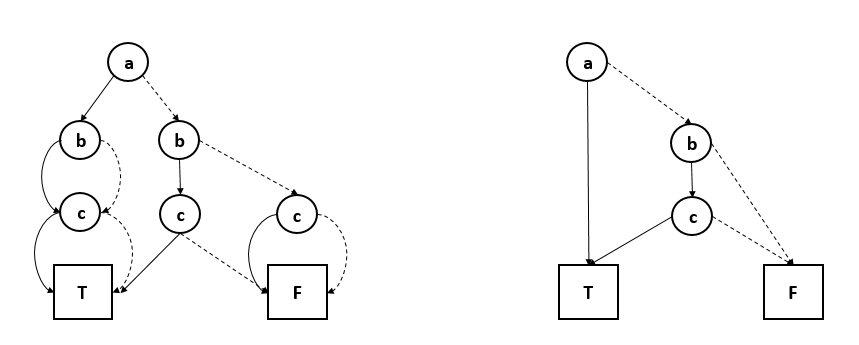
\includegraphics[width=0.8\textwidth] {images/bdd.png}}
        \caption{\label{fig:bdd} Binary Decision Diagrams of the Formula $a \lor (b \land c)$}
\end{figure}
As shown in Figure~\ref{fig:bdd}, it is a rooted, directed, acyclic graph with internal decision nodes and two terminal nodes (\textit{true} and \textit{false}). Each of the decision nodes is labeled with a Boolean variable and has two child nodes, low child and high child. The edge from a node to its low child represents the assignment of \textit{false}, likewise the edge to the high child represents the assignment of \textit{true}. The BDD is called \textit{ordered} if different variables appear in the same order on all paths from the root. Intuitively, following a path from the root to the \textit{true} terminal node represents a valid assignment to the Boolean formula (invalid in the case of ending on the \textit{false} terminal node). 

BDDs are reduced by the removal of isomorphic subgraphs. The BDD shown on the right of Figure~\ref{fig:bdd} is the reduced form of the BDD on the left.

\subsubsection{State Machines and Their Verification}
A finite state machine (or finite state automaton) is a mathematical model of computation and consists of states, represented by nodes, and transitions between them, represented by directed edges. The change from one state to another is called a {\em transition}. The abstract machine can be in exactly one of a finite number of states at a time (hence, finite). \danielle{make figure?}

An infinite state machine has much more power in representation due to the ability to deal with infinite states. In domains like model checking, this is required since many of the variables used are from infinite domains (e.g., real numbers, integers). The expressive capabilities of set notation and predicate logic allow finite strings to represent these infinite states. For example, the infinite set of integers greater than zero is described succintly as: $\{x \in \mathbb{Z} : x > 0\}$. 

Abstracting a program or system with respect to a state machine is great, but without being able to reason about that abstraction, it is nothing more than slightly interesting. Information commonly required of a state machine representation is if a given state is {\em reachable}. In other words, reachability determines if is there a sequence of transitions that can lead to a given state. 

Model checkers often utilize the expressive power of state machines to verify specifications. One such example important to this thesis is JKind~\cite{2017arXiv171201222G}, an infinite state model checker. Verification of the program is based on {\em k-induction} (see Section~\ref{subsubsec:kInd}) and property directed reachability using a back-end SMT solver, e.g., Z3~\cite{z3}, SMTInterpol~\cite{smtInterpol}.

\subsubsection{Transition Systems}
Informally, a transition system is a model of states and transitions between them. Intuitively, finite automata are like transition systems with additional constraints, for instance, defined start and final states. Transition systems are directed graphs with nodes representing reachable states and edges representing transitions between them. They may also be defined with a mapping function that assigns labels to each node; in the context of model checking, these labels are often properties which must hold in the corresponding state.

Labeled transition systems are used extensively in model checking and will be mentioned within that context in later sections. There is much that could be said about transition systems, but for the purpose of this body of work, it is unnecessary. More information about transition systems and their relation to safety analysis and model checking can be found in the comprehensive book written by Bozzano and Villafiorita, Design and Safety Assessment of Critical Systems~\cite{Bozzano:2010:DSA:1951720}.

\subsubsubsection{$k$-induction}
\label{subsubsec:kInd}
The $k$-induction method was introduced as a technique for SAT-based verification of finite and infinite state transition systems~\cite{sheeran2000checking}. Let $I(s)$ and $T(s, s_0)$ be formulae encoding the initial states and transition relation for a system over sets of propositional state variables $s$ and $s_0$. Additionally, let $P(s)$ be a formula that represents the states satisfying a safety property and $k$ a positive integer. To prove the safety property $P$ by $k$-induction, there are two steps, the base case and the induction case. The base case must show that $P$ holds in all states reachable from an initial state within $k$ steps, or transitions. More formally, the base case must show that the following formula is unsatisfiable:

\begin{center}
$I(s_1) \land T(s_1, s_2) \land \cdots \land T(s_{k−1}, s_k) \land (\overline{P(s_1)} \lor \cdots \lor \overline{P(s_k)})$
\end{center}

The induction step must show that whenever $P$ holds in $k$ consecutive states, $s_1, \ldots, s_k$, $P$ also holds in the next state $s_{k+1}$ of the system. This is done by showing that the step case formula is unsatisfiable:

\begin{center}
$P(s_1) \land T(s_1, s_2) \land \cdots \land P(s_k) \land T(s_{k}, s_{k+1}) \land \overline{P(s_{k+1})}$
\end{center}

Ever since $k$-induction was introduced for the purpose of verification of state machines, various methods came about of either combining these two proof steps into one~\cite{donaldson2011software} or performing them in parallel~\cite{kahsai2011pkind}. \\

\begin{center}
Said a fellow in liquor production\\
``I’ve a still of ingenious construction\\
the alcohol boils\\
through old magnet coils\\
I’ve dubbed it my Proof by Induction"\\
\textit{- Author unknown}
\end{center}

\subsubsubsection{Linear Temporal Logic}
Temporal logic can be used to express properties of reactive systems~\cite{Bozzano:2010:DSA:1951720}. System properties are usually classified into two main categories: {\em safety} properties and {\em liveness} properties. Safety properties express the idea that ``nothing bad ever happens" where liveness properties state that ``something good will eventually happen." 

An example of a safety property is: ``it is never the case that the brake pedal is pressed and no hydraulic pressure is supplied at the wheel." A liveness property, on the other hand, could state: ``eventually the process will complete it's execution." 

Traditionally, two types of temporal logic are used in model checking; Computational Tree Logic (CTL), which is based on a branching logic model, and Linear Temporal Logic (LTL), based on a linear representation of time. This research will focus on LTL. 

An LTL formula is built from a set of atomic propositions, logical operators, and basic temporal operators. The formula is evaluated over a linear path or sequence of states, $s_0, s_1, ..., s_i ,s_{i+1},...$. The following temporal operators are provided:
\begin{itemize}
    \item Globally (\textbf{G}): $G_p$ is true in a state $s_i$ if and only if $p$ is true in all states $s_j$ with $j \geq i$.
    
    \item Finally (\textbf{F}): $F_p$ is true in state $s_i$ if and only if $p$ is true in some state $s_j$ with $j \geq i$.
    
    \item Next (\textbf{X}): $X_p$ is true in state $s_i$ if and only if $p$ is true in the state $s_{i+1}$. 
    
    \item Until (\textbf{U}): $pUq$ is true in state $s_i$ if and only if $q$ is true in some state $s_j$ with $j \geq i$ and $p$ is true in all states $s_k$ such that $i \leq k < j$.
\end{itemize}

Other temporal operators can be defined on the basis of the operators above~\cite{sistla1985complexity}. Formal definitions and more information on LTL and CTL can be found in a number of research works~\cite{Bozzano:2010:DSA:1951720, clarke2018model}.

\subsection{Compositional Model Checking and AGREE}
\label{compModelChecking}
Compositional analysis of systems was introduced in order to address the scalability of model checking large software systems~\cite{pnueli1985transition, heckel1998compositional, NFM2012:CoGaMiWhLaLu}. Normally, a SAT solver will flatten the hierarchical system model and use all model elements from all layers in order to find proof of a safety property. The analysis can alternatively be performed compositionally following the architecture hierarchy such that analysis at a higher level is based on the components at the next lower level and conducted layer by layer; the components of a system are organized hierarchically and each layer of the architecture is viewed a system. The idea is to partition the formal analysis of a system architecture into verification tasks that correspond into the decomposition of the architecture. 

\subsubsection{Assume-Guarantee Reasoning Environment}
The Assume-Guarantee Reasoning Environment (AGREE)~\cite{cofer2012compositional} provides a way to perform compositional verification on models that are defined using the Architecture Analysis and Design Language (AADL)~\cite{aerospace2012sae}. 

A component contract in an assume-guarantee reasoning environment is an assume-guarantee pair. Intuitively, the meaning of a pair is: if the assumption is true, then the component will ensure that the guarantee is true. The formulation of AGREE uses LTL operators $G$ (globally), $H$ (historically), and $Z$ (in the previous instant).

Formally, a component contract is an assume-guarantee pair $(A,P)$ for propositions $A, P$. The meaning of a pair is that a component is required to meet it's guarantee only if its assumptions have been true up to the current instant~\cite{cofer2012compositional}. Stated as an LTL formula, this is $G(H(A) \implies P)$. 

Each architectural layer is viewed as a system with inputs, outputs, and components. A system $S$ can be described as its own contract $(A_S, P_S)$ and the contracts of its components $C_S$. Thus, $S = (A_S, P_S, C_S)$. For each layer, the proof consists of demonstrating that the system guarantee is provable given the guarantees of its direct subcomponents and the system assumptions, or more formally prove $G(H(A_S) \implies P_S)$ given $G(H(A_C) \implies P_C)$ for each component $C$ in the system.  

This proof is performed one layer at a time starting from the top level of the system. When compared to monolithic analysis (i.e., analysis of the flattened model composed of all components), the compositional approach allows the analysis to scale to much larger systems~\cite{NFM2012:CoGaMiWhLaLu}. AGREE utilizes the JKind model checker~\cite{2017arXiv171201222G}, an infinite state $k$-induction model checker. Verification of the program is performed using a back-end SMT solver, e.g., Z3~\cite{z3}, SMTInterpol~\cite{smtInterpol}. 
%\section{Formal Methods in Safety Analysis: A Brief History and the State of the Practice}
\label{sec:modelCheckingInSA}
Safety analysis has traditionally been performed manually, but with the rise of model checking and the improvement of its capabilities, the world of safety analysis began to see its powerful benefits~\cite{hinchey2012industrial, liggesmeyer1998improving, coudert1993fault, Bozzano:2010:DSA:1951720,bozzano2003esacs}. There arose multiple ways of viewing the system and fault models, various ways of automating the capture of safety pertinent information, and a number of tools that addressed various issues that arose. In this section, we discuss the state of the practice and how formal methods has been applied in the domain of safety assessment research.

\subsection{Model Checking in Model Based Safety Analysis}
From the beginnings of model checking, there was a slow increase in its application to the domain of safety analysis, but a few research groups contributed immensely to this branch of study. Separately, these researchers began to contribute to safety analysis through the use of model checking starting in the '90's and are still contributing today (e.g., \cite{reese1997software,signoret1998altarica,chiappini1999formal,cimatti2000industrial}. 

One of the main methods was the abstraction of the system into a formal transition system; this provided a means of defining a precise mathematical model of the system and simplifying mathematical operations through the use of abstraction techniques on the transition system. This helped to shrink the entire state space into something more digestible by computational techniques~\cite{d2008survey}. 

In the early 2000's, model based safety assessment began to make an appearance in literature~\cite{Bozzano:2010:DSA:1951720,Joshi05:Dasc, Joshi05:SafeComp, Joshi07:Hase}. This applied model checking and model based system development to safety analysis at the same time.  In this approach, a safety analysis system model (SASM) is the central artifact in the safety analysis process, and traditional safety analysis artifacts, such as fault trees, are automatically generated by tools that analyze the SASM.

The contents and structure of the SASM differ significantly across different conceptions of MBSA.  We can draw distinctions between approaches along several different axes.  The first is whether they propagate faults explicitly through user-defined propagations, which we call {\em failure logic modeling} (FLM), or {\em explicit propagation}, or through existing behavioral modeling, which we call {\em failure effect modeling} (FEM), or {\em implicit propagation}.  The next is whether models and notations are {\em purpose-built} for safety analysis vs. those that extend {\em existing system models} (ESM).

For FEM approaches, there are several additional dimensions.  One dimension involves whether {\em causal} or {\em non-causal} models are allowed.  Non-causal models allow simultaneous (in time) bi-directional error propagations, which allow more natural expression of some failure types (e.g. reverse flow within segments of a pipe), but are more difficult to analyze.  A final dimension involves whether analysis is {\em compositional} across layers of hierarchically-composed systems or {\em monolithic}.  %Our approach is an extension of AADL (ESM), causal, compositional, mixed FLM/FEM approach.
\danielle{Make a figure here - that will help explain these distinctions.}

This literature overview is not a complete account of all safety analysis model checking tools available either in industry or research, but highlights some of the most influential safety assessment methods and tools currently available. 

\subsubsection{AltaRica}
AltaRica was one of the first model checking tools specifically aimed at safety analysis of critical systems. The first iteration of AltaRica (1.0) performed over a transition system of the model, used dataflow ({\em causal}) semantics, and could capture the hierarchy of a system~\cite{signoret1998altarica}. The key idea was that this transition system (more specifically {\em constraint automata}) could be compiled into Boolean formulae and transformed into a BDD~\cite{point1999altarica}. The literature for performing fault tree analysis over BDDs was rich with algorithms; this was how much of the safety analysis artifacts were generated. The dataflow dialect (AltaRica 1.0) has substantial tool support, including the commercial Cecilia OCAS tool from Dassault~\cite{bieber2004safety}. For this dialect, the safety assessment, fault tree generation, and functional verification can be performed with the aid of NuSMV model checking~\cite{symbAltaRica}.

The most recent language update (AltaRica 3.0) uses non-causal semantics~\cite{prosvirnova2013compilationfaulttrees,PROSVIRNOVA2013127}. Failure states are defined throughout the system and flow variables are updated through the use of assertions~\cite{Bieber04safetyassessment}.  AltaRica 3.0 has support for simulation and Markov model generation through the OpenAltaRica (www.openaltarica.fr) tool suite; it is a {\em FEM}-based, {\em purpose-built}, {\em monolithic} safety analysis language. 

AltaRica 3.0 provides automated fault tree generation by translating the model into a reachability graph and then further compiling it into Boolean formula in order to compute minimal cut sets~\cite{prosvirnova2015automated}. 

\subsubsection{FSAP, xSAP, and COMPASS}
The Formal Safety Analysis Platform (FSAP) was introduced in 2003~\cite{bozzano2003improving} and supported failure mode definitions, safety requirements in temporal logic formulae, automated fault tree construction, and counterexample traces. The platform used NuSMV, a BDD-based model checker~\cite{Cimatti2000}. The system model, written in NuSMV, and the fault model, developed graphically in FSAP, are together translated into a finite state machine and eventually into a BDD; fault tree analysis is performed using BDD algorithms implemented in NuSMV. 

By 2016, the researchers that developed FSAP (Foundation Bruno Kessler, FBK) released a similar tool called xSAP~\cite{DBLP:conf/tacas/BittnerBCCGGMMZ16}. xSAP extends FSAP in many ways: xSAP can handle infinite state machines, it is textual language rather than graphical, allows for richer fault modeling and definitions, and implements more than just BDD computations (e.g., SAT- and SMT-based routines). xSAP was integrated into the COMPASS toolsuite to take advantage of the algorithms it supports. More complex SAT-based algorithms were introduced to bypass the BDD method of minimal cut set generation, namely the ``anytime approximation" algorithms~\cite{CAV2015:BoCiGrMa, mattarei2016scalable}. These algorithms make clever use of bounded model checking algorithms to explore counterexamples provided to the query "the top level event never occurs." These explorations are done such that the cut sets generated are of increasing cardinality which allows for an approximation computation to be given even when the state space is too large to compute all minimal cut sets. These are implemented in xSAP~\cite{CAV2015:BoCiGrMa}.

COMPASS (Correctness, Modeling project and Performance of Aerospace Systems)~\cite{10.1007/978-3-642-04468-7_15} is a mixed {\em FLM/FEM}-based, {\em causal} {\em compositional} tool suite that uses the SLIM language, which is based on a subset of the Architecture Analysis and Design Language (AADL), for its input models~\cite{5185388, criticalembeddedsystems}. In SLIM, a nominal system model and the error model are developed separately and then transformed into an extended system model.  This extended model is automatically translated into input models for the NuSMV model checker~\cite{Cimatti2000, NuSMV}, MRMC (Markov Reward Model Checker)~\cite{Katoen:2005:MRM:1114692.1115230, MRMC}, and RAT (Requirements Analysis Tool)~\cite{RAT}. The safety analysis tool xSAP~\cite{DBLP:conf/tacas/BittnerBCCGGMMZ16} can be invoked in order to generate safety analysis artifacts such as fault trees and FMEA tables~\cite{compass30toolset}.  %COMPASS is an impressive tool suite, but some of the features that make AADL suitable for SW/HW architecture specification: event and event-data ports, threads, and processes, appear to be missing, which means that the SLIM language may not be suitable as a general system design notation (ESM).

\subsubsection{SmartIFlow}
SmartIFlow~\cite{info17:HaLuHo,honig2014new} is a {\em FEM}-based, {\em purpose-built}, {\em monolithic} {\em non-causal} safety analysis tool that describes components and their interactions using finite state machines and events. Verification is done through an explicit state model checker which returns sets of counterexamples for safety requirements in the presence of failures.  SmartIFlow allows {\em non-causal} models containing simultaneous (in time) bi-directional error propagations.  On the other hand, the tools do not yet appear to scale to industrial-sized problems, as mentioned by the authors: ``As current experience is based on models with limited size, there is still a long way to go to make this approach ready for application in an industrial context''~\cite{info17:HaLuHo}.

\subsubsection{SAML}
The Safety Analysis and Modeling Language (SAML)~\cite{Gudemann:2010:FQQ:1909626.1909813} is a {\em FEM}-based, {\em purpose-built}, {\em monolithic} {\em causal} safety analysis language that was developed in 2010.  System models constructed in SAML can be used used for both qualitative and quantitative analyses. It allows for the combination of discrete probability distributions and non-determinism. The SAML model can be automatically imported into several analysis tools like NuSMV~\cite{Cimatti2000}, PRISM (Probabilistic Symbolic Model Checker)~\cite{CAV2011:KwNoPa}, or the MRMC probabilistic model checker~\cite{Katoen:2005:MRM:1114692.1115230}. SAML itself does not provide the formal verification engines, but instead provides a platform to model the safety aspects of a system and then translate this into the input language for a formal verification engine~\cite{Gudemann:2010:FQQ:1909626.1909813}.

\subsubsection{Error Model Annex for AADL}
The SAE (Society of Automotive Engineers) released the
aerospace standard AS5506, named Architecture Analysis and Design Language (AADL), which is a mature industry-standard for embedded systems and has proved to be efficient for architecture modeling~\cite{aerospace2012sae,liu2016research}. AADL supports safety analysis by adding EMA (Error Model Annex) as an extension to the language. EMA allows the user to annotate system hardware and software architectures with hazard, error propagation, failure modes and effects due to failures. Around 2016, Version 2 of the Error Model Annex was released (EMV2)~\cite{EMV2}. EMV2 is an {\em FLM}-based {\em ESM} approach. The faults and error propagations are explicitly defined and the fault tree analysis is performed by traversing propagation paths in reverse to find the original fault that caused the problem~\cite{feiler2017automated}. 


